\documentclass[conference]{IEEEtran}
\usepackage{cite}
\usepackage{amsmath,amssymb}
\usepackage{graphicx}
\usepackage{booktabs}
\usepackage{url}
\usepackage{tikz}
\usetikzlibrary{positioning,arrows.meta}
\graphicspath{{figures/}}
\makeatletter
\@namedef{v@abl.minilm.title}{0.468}
\@namedef{v@abl.minilm.titleloss}{0.057}
\@namedef{v@abl.sparse.best.ta}{0.459}
\@namedef{v@abl.titleloss}{0.057--0.125}
\@namedef{v@ai.disclosure}{Generative AI (Claude, Anthropic) was used to help write the analysis scripts and edit the manuscript text. The authors designed the study, ran all experiments, produced the manual relevance labels, verified all code, results and references, and take full responsibility for the content.}
\@namedef{v@gap.points}{6.4}
\@namedef{v@gap.points.y}{8.6}
\@namedef{v@main.sentence}{Among the dense encoders, SPECTER2 is first on the May corpus and SPECTER2 on the 2020--2024 corpus; the best sparse system is BM25 on both.}
\@namedef{v@may.BGE.MRR}{0.684}
\@namedef{v@may.BGE.P5}{0.512}
\@namedef{v@may.BGE.gap}{+0.056}
\@namedef{v@may.BGE.nDCG}{0.466}
\@namedef{v@may.BM25.MRR}{0.647}
\@namedef{v@may.BM25.P5}{0.456}
\@namedef{v@may.BM25.nDCG}{0.440}
\@namedef{v@may.Hyb.MRR}{0.684}
\@namedef{v@may.Hyb.P5}{0.509}
\@namedef{v@may.Hyb.nDCG}{0.469}
\@namedef{v@may.LSA.MRR}{0.627}
\@namedef{v@may.LSA.P5}{0.454}
\@namedef{v@may.LSA.nDCG}{0.437}
\@namedef{v@may.MiniLM.MRR}{0.679}
\@namedef{v@may.MiniLM.P5}{0.510}
\@namedef{v@may.MiniLM.gap}{+0.054}
\@namedef{v@may.MiniLM.nDCG}{0.467}
\@namedef{v@may.SPECTER.MRR}{0.685}
\@namedef{v@may.SPECTER.P5}{0.520}
\@namedef{v@may.SPECTER.gap}{+0.064}
\@namedef{v@may.SPECTER.nDCG}{0.474}
\@namedef{v@may.TFIDF.MRR}{0.618}
\@namedef{v@may.TFIDF.P5}{0.429}
\@namedef{v@may.TFIDF.nDCG}{0.418}
\@namedef{v@may.authorfilter.maxdiff}{0.008}
\@namedef{v@may.best.P5}{0.520}
\@namedef{v@may.best.name}{SPECTER2}
\@namedef{v@may.chance}{0.196}
\@namedef{v@may.curve.best}{0.472}
\@namedef{v@may.curve.spread}{0.003}
\@namedef{v@may.hyb.diff}{$-$0.001}
\@namedef{v@may.hyb.p}{0.95}
\@namedef{v@may.hybtuned.P5}{0.516}
\@namedef{v@may.hybtuned.w}{0.8}
\@namedef{v@may.neardup}{34--46}
\@namedef{v@may.ov.MiniLM.BM25}{0.13}
\@namedef{v@may.ov.MiniLM.LSA}{0.12}
\@namedef{v@may.ov.dense}{0.20--0.26}
\@namedef{v@may.rrf.nDCG}{0.471}
\@namedef{v@may.sharedauthor}{1.5--2.9\%}
\@namedef{v@may.slots}{41{,}840}
\@namedef{v@may.spec.minilm}{+0.010}
\@namedef{v@may.spec.minilm.p}{0.004}
\@namedef{v@may.test}{8{,}368}
\@namedef{v@pool.size}{212}
\@namedef{v@reader.hi}{0.20}
\@namedef{v@reader.lo}{0.10}
\@namedef{v@reader.nodense}{9}
\@namedef{v@reader.onlydense}{1}
\@namedef{v@reader.rel}{18}
\@namedef{v@reader.sentence}{Of the 212 pooled candidates the first author marked 18 as the same research problem; for 2 of the ten queries no pooled candidate qualified. Reader P@5 is low for every system, between 0.10 and 0.20, and it does not follow the ranking by category: BM25, TF-IDF and the hybrid reach 0.18--0.20, while LSA, MiniLM and SPECTER2 reach 0.10. Of the 18 same-problem papers, 9 were retrieved by none of the three dense encoders and 1 only by them. Category agreement over-counts far more often than it under-counts: of the 150 top-five slots of the dense encoders, 79 share the query's category without addressing the same problem, while 13 address the same problem from another category. With ten queries and one annotator these figures are descriptive, but they indicate that the dense advantage in category precision reflects topical closeness more than same-problem relevance.}
\@namedef{v@repo}{Armani7777/arxiv-similar-paper-retrieval}
\@namedef{v@tune.bestsparse.y}{0.491}
\@namedef{v@tune.maxgain}{0.033}
\@namedef{v@tune.maxgain.y}{0.039}
\@namedef{v@y.BGE.MRR}{0.695}
\@namedef{v@y.BGE.P5}{0.542}
\@namedef{v@y.BGE.gap}{+0.061}
\@namedef{v@y.BGE.nDCG}{0.506}
\@namedef{v@y.BM25.MRR}{0.662}
\@namedef{v@y.BM25.P5}{0.481}
\@namedef{v@y.BM25.nDCG}{0.460}
\@namedef{v@y.Hyb.MRR}{0.705}
\@namedef{v@y.Hyb.P5}{0.548}
\@namedef{v@y.Hyb.nDCG}{0.503}
\@namedef{v@y.LSA.MRR}{0.633}
\@namedef{v@y.LSA.P5}{0.467}
\@namedef{v@y.LSA.nDCG}{0.458}
\@namedef{v@y.MiniLM.MRR}{0.708}
\@namedef{v@y.MiniLM.P5}{0.561}
\@namedef{v@y.MiniLM.gap}{+0.080}
\@namedef{v@y.MiniLM.nDCG}{0.509}
\@namedef{v@y.SPECTER.MRR}{0.711}
\@namedef{v@y.SPECTER.P5}{0.567}
\@namedef{v@y.SPECTER.gap}{+0.086}
\@namedef{v@y.SPECTER.nDCG}{0.515}
\@namedef{v@y.TFIDF.MRR}{0.623}
\@namedef{v@y.TFIDF.P5}{0.452}
\@namedef{v@y.TFIDF.nDCG}{0.434}
\@namedef{v@y.authorfilter.maxdiff}{0.005}
\@namedef{v@y.candidates}{10{,}710}
\@namedef{v@y.chance}{0.165}
\@namedef{v@y.curve.best}{0.510}
\@namedef{v@y.curve.spread}{0.008}
\@namedef{v@y.hyb.diff}{$-$0.013}
\@namedef{v@y.hyb.p}{$<$0.002}
\@namedef{v@y.hybtuned.P5}{0.561}
\@namedef{v@y.hybtuned.w}{0.9}
\@namedef{v@y.neardup}{74--106}
\@namedef{v@y.ov.dense}{0.24--0.30}
\@namedef{v@y.rrf.nDCG}{0.504}
\@namedef{v@y.sharedauthor}{1.4--2.8\%}
\@namedef{v@y.slots}{42{,}485}
\@namedef{v@y.spec.minilm}{+0.006}
\@namedef{v@y.spec.minilm.p}{0.014}
\@namedef{v@y.test}{8{,}497}
\@namedef{v@y.weakestdense.P5}{0.542}
\makeatother
\newcommand{\val}[1]{\ifcsname v@#1\endcsname\csname v@#1\endcsname\else\textbf{??#1??}\fi}


\begin{document}

\title{Comparative Analysis of Vectorization Models and Retrieval Methods for Finding Similar Scientific Papers}

\author{
\IEEEauthorblockN{Arman Tursynbayev}
\IEEEauthorblockA{School of Computer Science\\
Astana IT University\\
Astana, Kazakhstan\\
armani7775@gmail.com}
\and
\IEEEauthorblockN{Zhanna Sadirmekova}
\IEEEauthorblockA{School of Computer Science\\
Astana IT University\\
Astana, Kazakhstan\\
Zhanna.Sadirmekova1@astanait.edu.kz}
}

\maketitle

\begin{abstract}
Literature search often starts from one paper: the reader has a relevant article and wants others on the same problem. We compare widely used text representations for this query-by-document task on arXiv computer-science preprints: BM25, TF-IDF, latent semantic analysis (LSA), three pretrained dense encoders (all-MiniLM-L6-v2, SPECTER2 and BGE-small) and a BM25--dense hybrid. Two corpora of 10{,}000 papers were collected through the arXiv API, one covering three weeks of May 2026 and one sampled across 2020--2024. Every eligible paper serves as a query with itself removed from the candidates; 1{,}000 queries per corpus are reserved for parameter selection and the remaining \val{may.test} and \val{y.test} for testing. A retrieved paper counts as relevant when it shares the query's primary arXiv category, a label that no compared system computes. All three dense encoders beat every sparse baseline on both corpora, also after the baselines are tuned: on the May corpus P@5 is \val{may.SPECTER.P5} for SPECTER2, \val{may.BGE.P5} for BGE-small and \val{may.MiniLM.P5} for MiniLM against \val{may.BM25.P5} for BM25, and the differences are significant under paired randomization tests with Holm correction. A tuned BM25 component adds little to a dense score. A blind problem-level reading of 10 queries by the first author tells a different story: same-problem precision is low for every system (\val{reader.lo}--\val{reader.hi}) and the dense encoders are not ahead, so category precision measures topical closeness rather than usefulness to a reader.
\end{abstract}

\begin{IEEEkeywords}
similar-paper search, query by document, BM25, latent semantic analysis, sentence embeddings, SPECTER2, hybrid retrieval, arXiv
\end{IEEEkeywords}

\section{Introduction}

A common way to explore a research topic is to start from one paper and ask for more like it. Digital libraries expose this as ``related articles'' or ``similar papers,'' and intelligent services that organize access to scientific and educational resources rely on the same operation \cite{batyrkhanov2022intelligent,serikbayeva2021access}. The engineering choice behind it is usually between a lexical ranker such as BM25 \cite{robertson2009bm25}, a vector-space or latent-semantic representation \cite{salton1988term,deerwester1990lsa}, and a pretrained dense encoder \cite{reimers2019sbert,cohan2020specter}. Published comparisons do not settle the choice. On heterogeneous retrieval benchmarks BM25 and dense models trade the lead from task to task \cite{thakur2021beir,muennighoff2023mteb}, and on large citation-recommendation pools BM25 remained competitive with transformer article encoders \cite{medic2022large}.

Evaluating similar-paper search also has a labeling problem. Expert relevance judgments for paper-to-paper similarity are expensive and exist for only a few hundred queries \cite{mysore2021csfcube}. Two cheaper shortcuts are common and both bias the result. If ``relevant'' is defined as ``close under an embedding,'' that embedding wins by construction. If the source paper stays in the index and the query is a fragment of its title, every ranker retrieves the source paper at rank one and reciprocal rank says little about the rest of the list. We avoid both: the query paper is removed from its own candidate list, and relevance is the primary arXiv category, which authors and moderators assign and which none of the compared systems computes.

This paper is an empirical comparison, not a new ranking model. Its contributions are:
\begin{itemize}
\item a controlled comparison of seven retrieval configurations on two arXiv corpora, a recent three-week slice and a five-year sample, using every eligible paper as a query rather than a small sample;
\item a sensitivity and ablation analysis covering BM25 $k_1$ and $b$, TF-IDF weighting, LSA rank, the hybrid weight and score normalization, and the text fields, with all choices made on a held-out query set;
\item paired significance tests with bootstrap confidence intervals for every headline difference;
\item a blind, problem-level reading of pooled results that measures how often the category proxy and same-problem relevance disagree.
\end{itemize}
Code, query lists, per-query scores and the manual labels are publicly released (see Data and Code Availability).

\section{Related Work}

\textit{Paper recommendation and scientific document representations.} Surveys of paper recommender systems group them into content-based, collaborative and graph-based families and note that evaluation protocols differ widely between studies \cite{kreutz2022survey,pinedo2025survey}. Among content-based encoders, SPECTER trains on citation triplets \cite{cohan2020specter}, SciNCL samples training pairs from citation-graph neighborhoods \cite{ostendorff2022scincl}, and SPECTER2 adds task-format adapters after SciRepEval showed that one embedding is a poor compromise across scientific tasks \cite{singh2023scirepeval}. ASPIRE matches papers through several aspect vectors \cite{mysore2022aspire}, and CSFCube provides faceted expert judgments for query-by-document search in computer science \cite{mysore2021csfcube}. LitSearch, a recent benchmark of literature-search questions, reports a large recall gap between BM25 and modern dense retrievers \cite{ajith2024litsearch}; its queries are natural-language questions, whereas ours are whole papers.

\textit{Lexical versus dense retrieval.} BEIR showed that zero-shot dense retrievers do not uniformly beat BM25 \cite{thakur2021beir}. MTEB and its multilingual extension MMTEB find that no single embedding model leads on all tasks \cite{muennighoff2023mteb,enevoldsen2025mmteb}. General-purpose encoders such as BGE are trained on large weakly supervised pair collections \cite{xiao2024cpack}, while compact models such as MiniLM are distilled from larger transformers \cite{wang2020minilm} and fine-tuned as sentence encoders \cite{reimers2019sbert}.

\textit{Hybrid retrieval.} Sparse and dense scores are often combined because they miss different documents \cite{luan2021sparse}. Bruch et al. show that a tuned convex combination of normalized scores usually outperforms reciprocal rank fusion (RRF) and that the result is fairly insensitive to the normalization choice \cite{bruch2022fusion}; RRF itself combines ranks rather than scores \cite{cormack2009rrf}. We test both, with the weight chosen on held-out queries.

\section{Data}
\label{sec:data}

Both corpora were downloaded with the \texttt{arxiv} Python client from the public arXiv API using the query \texttt{cat:cs.AI OR cat:cs.LG OR cat:cs.CL OR cat:cs.IR}. Each record keeps the identifier, title, abstract, author list, category list, primary category, and first-version and latest-version dates. The category list stores the \texttt{cs.*} tags of a paper; the primary category is stored even when it lies outside computer science, so cross-listed papers such as \texttt{stat.ML} or \texttt{eess.IV} keep their own primary label.

\textit{May 2026 corpus.} This is the collection used in the submitted version of this study: the 10{,}000 most recent matching records returned on 31~May~2026, sorted by submission date, with publication dates from 5 to 28~May~2026. The API stopped returning pages at 10{,}000 records.

\textit{2020--2024 corpus.} To test whether the results depend on a three-week window, we built a second corpus. Each month of 2020--2024 was split into four windows starting on days 1, 8, 15 and 22, and the first 45 papers by submission date were taken from each window. Of the 240 windows, the two covering 1--14 January 2024 failed with HTTP~429 rate-limit responses and were not retried, so that the stored sample is not changed after it was drawn. After removing 90 duplicates, \val{y.candidates} candidates remained and 10{,}000 were kept by a seeded uniform draw.

Table~\ref{tab:data} summarizes both files. Neither contains a paper twice under different version suffixes, every record has a publication date inside its stated range, and every abstract consists of at least 90\% ASCII letters, so no language filter was needed. Two kinds of near-duplicate hits could inflate precision: papers by the same authors and near-identical texts. Across all systems, \val{may.sharedauthor} of the \val{may.slots} top-five slots of the May test queries share at least one author name with the query (\val{y.sharedauthor} for 2020--2024), and \val{may.neardup} slots per system have a title-word Jaccard of 0.5 or more with the query. Both effects are too small to change the comparison.

\begin{table}[!t]
\centering
\caption{The two corpora.}
\label{tab:data}
\footnotesize
\setlength{\tabcolsep}{3pt}
\begin{tabular}{@{}lcc@{}}
\toprule
 & May 2026 & 2020--2024 \\
\midrule
Records & 10{,}000 & 10{,}000 \\
Publication dates & 2026-05-05 -- 05-28 & 2020-01 -- 2024-12 \\
Distinct primary categories & 107 & 104 \\
Primary in query categories & 69.2\% & 59.7\% \\
\quad cs.LG / cs.CL & 34.6\% / 15.7\% & 32.1\% / 17.9\% \\
\quad cs.AI / cs.CV & 16.7\% / 9.3\% & 6.2\% / 11.4\% \\
Categories per paper (mean) & 1.79 & 1.87 \\
Abstract words (median) & 194 & 175 \\
Revised after v1 & 11.3\% & 42.0\% \\
Queries: eligible/dev/test & 9{,}368/1{,}000/8{,}368 & 9{,}497/1{,}000/8{,}497 \\
Chance precision (test) & 0.196 & 0.165 \\
\bottomrule
\end{tabular}
\end{table}


\textit{Queries and splits.} A paper is eligible as a query when its primary category has at least 30 papers in the corpus, so that five same-category hits remain possible. From the eligible papers, 1{,}000 are drawn with seed 43 as a development set; they are used only to choose parameters. All other eligible papers form the test set, and every number in the main tables comes from it.

\section{Retrieval Methods}
\label{sec:methods}

All systems index the concatenation of title and abstract. For a query paper $q$ the candidates are $\mathcal{C}_q = \mathcal{D}\setminus\{q\}$, and each system returns the top 100 candidates.

\textit{BM25} \cite{robertson2009bm25} scores a candidate $d$ as
\begin{equation}
s(q,d)=\sum_{t\in q}\mathrm{idf}(t)\,\frac{f_{t,d}\,(k_1+1)}{f_{t,d}+k_1\!\left(1-b+b\,|d|/\overline{|d|}\right)},
\label{eq:bm25}
\end{equation}
with $\mathrm{idf}(t)=\ln\!\left(1+\frac{N-n_t+0.5}{n_t+0.5}\right)$, where $f_{t,d}$ is the frequency of term $t$ in $d$, $n_t$ the number of documents containing $t$, and $N$ the corpus size. Each distinct query term is counted once. Tokens are lowercase alphanumeric strings longer than two characters, excluding the scikit-learn English stop list and pure numbers. The defaults $k_1=1.5$ and $b=0.75$ follow common toolkits \cite{lin2021pyserini}.

\textit{TF-IDF} \cite{salton1988term} uses scikit-learn with the same stop list, terms in at least 3 and at most 90\% of documents, and at most 20{,}000 terms; vectors are L2-normalized and compared by cosine similarity.

\textit{LSA} \cite{deerwester1990lsa} applies truncated SVD, $X\approx U_k\Sigma_kV_k^{\top}$, to the TF-IDF matrix and represents each paper by its L2-normalized row of $U_k\Sigma_k$; the default rank is $k=128$.

\textit{Dense encoders.} We use three public checkpoints without fine-tuning: \texttt{all-MiniLM-L6-v2} (384 dimensions, input truncated at 256 word pieces) \cite{wang2020minilm,reimers2019sbert}; SPECTER2 with its proximity adapter (768 dimensions, title and abstract joined by the separator token, 512 word pieces, CLS pooling) \cite{singh2023scirepeval}; and \texttt{bge-small-en-v1.5} (384 dimensions, 512 word pieces) \cite{xiao2024cpack}. Vectors are L2-normalized and ranked by cosine similarity.

\textit{Hybrid.} The hybrid score combines a dense score and BM25:
\begin{equation}
h(q,d)=w\,\hat{s}_{\mathrm{dense}}(q,d)+(1-w)\,\hat{s}_{\mathrm{BM25}}(q,d),
\label{eq:hybrid}
\end{equation}
where $\hat{s}$ is min-max normalized over $\mathcal{C}_q$. The pre-specified configuration is MiniLM with $w=0.6$, the value fixed in the configuration of our earlier prototype. In the sensitivity analysis we also vary $w$ from 0 to 1, replace min-max by z-score normalization, and test RRF with constant 60 \cite{cormack2009rrf}. Unlike the submitted version, normalization now excludes the query paper itself; including it compressed the BM25 component, because a paper's BM25 score against itself is far larger than against any other paper.

Fig.~\ref{fig:pipeline} summarizes the pipeline.

\begin{figure}[!t]
\centering
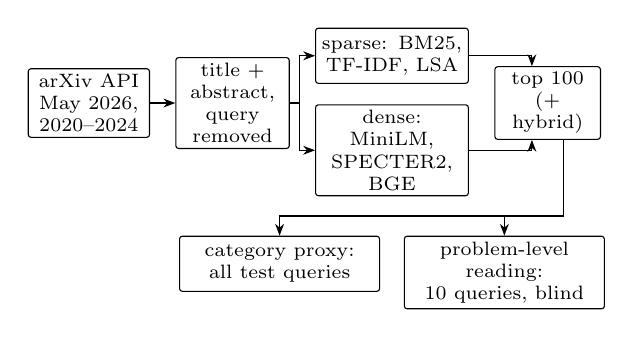
\begin{tikzpicture}[font=\scriptsize, node distance=2.2mm and 3.2mm,
  box/.style={draw, rounded corners=1pt, align=center, inner sep=2pt, minimum height=7mm, text width=#1},
  box/.default=15mm,
  arr/.style={-{Stealth[length=1.5mm]}}]
\node[box=14mm] (api) {arXiv API\\May 2026,\\2020--2024};
\node[box=13mm, right=of api] (txt) {title +\\abstract,\\query removed};
\node[box=18mm, right=of txt, yshift=6mm] (sp) {sparse: BM25,\\TF-IDF, LSA};
\node[box=18mm, right=of txt, yshift=-6mm] (de) {dense: MiniLM,\\SPECTER2, BGE};
\node[box=12mm] (hy) at ([xshift=10mm]sp.east |- txt) {top 100\\(+ hybrid)};
\node[box=24mm, anchor=north east] (cat) at ([yshift=-5mm, xshift=-1.5mm]de.south) {category proxy:\\all test queries};
\node[box=24mm, anchor=north west] (man) at ([yshift=-5mm, xshift=1.5mm]de.south) {problem-level reading:\\10 queries, blind};
\draw[arr] (api) -- (txt);
\draw[arr] (txt.east) -- ++(1.2mm,0) |- (sp.west);
\draw[arr] (txt.east) -- ++(1.2mm,0) |- (de.west);
\draw[arr] (sp.east) -| ([xshift=-2mm]hy.north);
\draw[arr] (de.east) -| ([xshift=-2mm]hy.south);
\coordinate (j) at ([yshift=-2.5mm]de.south -| hy.south);
\draw ([xshift=2mm]hy.south) |- (j);
\draw[arr] (j) -| (cat.north);
\draw[arr] (j) -| (man.north);
\end{tikzpicture}
\caption{Evaluation pipeline. The query paper is removed from its own candidate list before ranking.}
\label{fig:pipeline}
\end{figure}

\section{Evaluation Protocol}
\label{sec:eval}

\textit{Relevance proxy.} A candidate is relevant when its primary category equals the query's. We use this label because it is available for every paper, so all test queries can be scored, and because no compared system produces it. It is an imperfect proxy for ``the same research problem'': a paper on the same problem can be filed under another category, and two papers in one category can address different problems. The problem-level reading below measures both failure modes directly.

\textit{Metrics.} Precision at $k$ is the fraction of the top $k$ that is relevant; we report $k=5$ and $k=10$. Mean reciprocal rank (MRR) uses the rank of the first relevant candidate within the top 100. For nDCG@10 the gain is graded, $g(q,d)=|C_q\cap C_d|/|C_q\cup C_d|$, the Jaccard overlap of the two category lists, and
\begin{equation}
\mathrm{nDCG@10}=\frac{1}{Z_q}\sum_{i=1}^{10}\frac{2^{g(q,d_i)}-1}{\log_2(i+1)},
\label{eq:ndcg}
\end{equation}
where $Z_q$ is the same sum for the ten candidates with the largest gain. A random ranking would reach an expected precision of $(n_c-1)/(N-1)$ for a query in category $c$ of size $n_c$; averaged over the test queries this chance level is \val{may.chance} for May 2026 and \val{y.chance} for 2020--2024.

\textit{Statistics.} For each pair of systems we compute per-query differences, a 95\% bootstrap interval of the mean difference (10{,}000 resamples), and a two-sided paired randomization test with 10{,}000 sign flips, which is well suited to retrieval metrics \cite{smucker2007significance}. Within each metric, $p$-values are adjusted with the Holm procedure \cite{holm1979}. With 10{,}000 permutations the smallest attainable $p$ is about $10^{-4}$.

\textit{Problem-level reading.} Ten test queries from the May corpus were drawn, one from each of the ten most frequent primary categories in the test set (seed 11). The top five of all seven systems were pooled, giving \val{pool.size} distinct candidates. The first author read the title and abstract of each query and candidate and marked a candidate relevant if it studies the same research problem: the same task applied to the same kind of object, a paper one would expect to cite in the related-work section. A shared field or technical term was not sufficient. The pool was shuffled, and neither the retrieving system nor any arXiv category was shown. Reader P@5 is the share of a system's own top five marked relevant; every top-five candidate is in the pool, so no hit is unjudged. This is a single-annotator check of the proxy, not a test collection.

\section{Results}
\label{sec:results}

\subsection{Main comparison}

Table~\ref{tab:main} gives the test-set results with pre-specified parameters. On both corpora each of the three dense encoders is ahead of each sparse baseline, and every system is far above the chance level. SPECTER2, the only encoder trained on scientific citations, is first on both corpora, but its lead over MiniLM is small (\val{may.spec.minilm} and \val{y.spec.minilm} P@5). BGE-small matches MiniLM on the May corpus and falls behind it on the 2020--2024 corpus. Among the sparse systems BM25 is best on both corpora; LSA is close to BM25 and clearly ahead of the TF-IDF matrix it is computed from.

\begin{table}[!t]
\centering
\caption{Test-set results with pre-specified parameters. Relevance: same primary category; nDCG@10 uses graded category overlap. Every 95\% interval for P@5 and nDCG@10 has a half-width of at most 0.007. Best value per column in bold.}
\label{tab:main}
\footnotesize
\setlength{\tabcolsep}{3.2pt}
\begin{tabular}{@{}lcccccc@{}}
\toprule
 & \multicolumn{3}{c}{May 2026} & \multicolumn{3}{c}{2020--2024} \\
\cmidrule(lr){2-4}\cmidrule(l){5-7}
Method & P@5 & nDCG@10 & MRR & P@5 & nDCG@10 & MRR \\
\midrule
BM25 & 0.456 & 0.440 & 0.647 & 0.481 & 0.460 & 0.662 \\
TF-IDF & 0.429 & 0.418 & 0.618 & 0.452 & 0.434 & 0.623 \\
LSA & 0.454 & 0.437 & 0.627 & 0.467 & 0.458 & 0.633 \\
\midrule
MiniLM & 0.510 & 0.467 & 0.679 & 0.561 & 0.509 & 0.708 \\
SPECTER2 & \textbf{0.520} & \textbf{0.474} & \textbf{0.685} & \textbf{0.567} & \textbf{0.515} & \textbf{0.711} \\
BGE-small & 0.512 & 0.466 & 0.684 & 0.542 & 0.506 & 0.695 \\
\midrule
Hybrid (0.6) & 0.509 & 0.469 & 0.684 & 0.548 & 0.503 & 0.705 \\
\bottomrule
\end{tabular}
\end{table}


The paired tests in Table~\ref{tab:stats} show that the advantage of each dense encoder over the best sparse baseline is small in absolute terms but precisely estimated: with more than 8{,}000 paired queries the bootstrap intervals exclude zero and the Holm-adjusted $p$-values are at the permutation floor. The pre-specified MiniLM hybrid ($w=0.6$) is indistinguishable from MiniLM on the May corpus (\val{may.hyb.diff}, $p_{\mathrm{Holm}}=\val{may.hyb.p}$) and slightly worse on the 2020--2024 corpus (\val{y.hyb.diff}, $p_{\mathrm{Holm}}\val{y.hyb.p}$). BM25 is ahead of TF-IDF on both corpora, a difference that the 100-query sample of the submitted version could not resolve; that sample also underestimated BM25, whose P@5 on it was 0.386.

\begin{table*}[!t]
\centering
\caption{Paired differences in test P@5: mean difference, 95\% bootstrap interval and Holm-adjusted randomization $p$-value.}
\label{tab:stats}
\footnotesize
\setlength{\tabcolsep}{5pt}
\begin{tabular}{@{}lcccc@{}}
\toprule
 & \multicolumn{2}{c}{May 2026} & \multicolumn{2}{c}{2020--2024} \\
\cmidrule(lr){2-3}\cmidrule(l){4-5}
Comparison & $\Delta$ [95\% CI] & $p$ & $\Delta$ [95\% CI] & $p$ \\
\midrule
MiniLM -- BM25 & +0.054 [+0.048, +0.060] & $<$0.002 & +0.080 [+0.074, +0.085] & $<$0.002 \\
SPECTER2 -- BM25 & +0.064 [+0.058, +0.070] & $<$0.002 & +0.086 [+0.080, +0.092] & $<$0.002 \\
BGE-small -- BM25 & +0.056 [+0.050, +0.062] & $<$0.002 & +0.061 [+0.055, +0.067] & $<$0.002 \\
SPECTER2 -- MiniLM & +0.010 [+0.004, +0.015] & 0.004 & +0.006 [+0.001, +0.011] & 0.014 \\
BGE-small -- MiniLM & +0.002 [$-$0.003, +0.007] & 0.946 & $-$0.019 [$-$0.023, $-$0.014] & $<$0.002 \\
BGE-small -- SPECTER2 & $-$0.008 [$-$0.013, $-$0.002] & 0.016 & $-$0.025 [$-$0.030, $-$0.020] & $<$0.002 \\
Hybrid (0.6) -- MiniLM & $-$0.001 [$-$0.006, +0.004] & 0.946 & $-$0.013 [$-$0.017, $-$0.009] & $<$0.002 \\
TF-IDF -- BM25 & $-$0.027 [$-$0.033, $-$0.021] & $<$0.002 & $-$0.029 [$-$0.035, $-$0.023] & $<$0.002 \\
LSA -- TF-IDF & +0.024 [+0.018, +0.030] & $<$0.002 & +0.015 [+0.009, +0.021] & $<$0.002 \\
\bottomrule
\end{tabular}
\end{table*}


The result lists overlap little. On the May corpus the mean Jaccard overlap of the top 10 is \val{may.ov.MiniLM.BM25} between MiniLM and BM25, \val{may.ov.MiniLM.LSA} between MiniLM and LSA, and only \val{may.ov.dense} among the three dense encoders, so systems with similar precision still return largely different papers.

\subsection{Per-category results}

Table~\ref{tab:bycat} splits P@5 for the four largest query categories of the May corpus. The gap between sparse and dense systems is smallest in \texttt{cs.LG} and \texttt{cs.AI}, where precision is bounded by heavy cross-listing, and largest in \texttt{cs.CL} and \texttt{cs.CV}, where task names and model names recur across categories and term matching alone attracts off-category papers.

\begin{table}[!t]
\centering
\caption{Test P@5 by primary category of the query, May 2026 corpus. Chance is $(n_c-1)/(N-1)$.}
\label{tab:bycat}
\scriptsize
\setlength{\tabcolsep}{2.8pt}
\begin{tabular}{@{}lrrrrrrrr@{}}
\toprule
Cat. & $n$ & Chance & BM25 & TF-IDF & LSA & MiniLM & SPEC2 & BGE \\
\midrule
cs.LG & 3{,}078 & 0.346 & 0.577 & 0.560 & 0.591 & 0.608 & \textbf{0.627} & 0.616 \\
cs.AI & 1{,}509 & 0.167 & 0.327 & 0.314 & 0.328 & 0.362 & 0.378 & \textbf{0.386} \\
cs.CL & 1{,}405 & 0.157 & 0.441 & 0.428 & 0.442 & \textbf{0.540} & 0.527 & 0.532 \\
cs.CV & 821 & 0.093 & 0.518 & 0.444 & 0.484 & \textbf{0.648} & 0.637 & 0.586 \\
\bottomrule
\end{tabular}
\end{table}


\subsection{Sensitivity, ablation and hybrid weights}

Table~\ref{tab:sens} reports development-set results for the parameter grids and the configuration selected by nDCG@10, scored once on the test set. Tuning moves the sparse baselines by at most \val{tune.maxgain} in test P@5, and no tuned sparse configuration reaches the weakest dense encoder. TF-IDF benefits most, from sublinear term frequency. For LSA, lower ranks are slightly better on this task, so the 128-dimensional default is not handicapped by too few components. The field ablation shows that the abstract carries most of the signal: title-only indexing loses \val{abl.titleloss} in dev P@5 for the sparse systems and \val{abl.minilm.titleloss} for MiniLM. Even from titles alone MiniLM (\val{abl.minilm.title}) is above every sparse system indexed on title and abstract (at most \val{abl.sparse.best.ta}).

\begin{table*}[!t]
\centering
\caption{Sensitivity on the 1{,}000 development queries (May 2026). Range: dev nDCG@10 across the grid. The configuration with the best dev nDCG@10 is then scored once on the test set (P@5, default $\rightarrow$ selected). Bottom: dev P@5 by indexed field.}
\label{tab:sens}
\footnotesize
\setlength{\tabcolsep}{5pt}
\begin{tabular}{@{}llccc@{}}
\toprule
System & Grid & Dev range & Selected & Test P@5 \\
\midrule
BM25 & $k_1\!\in\!\{0.9,1.2,1.5,2\}$, $b\!\in\!\{.4,.6,.75,.9\}$ & 0.429--0.437 & k1=2.0, b=0.9 & 0.456 $\rightarrow$ 0.460 \\
TF-IDF & min\_df$\in\!\{1,3,5\}$, sublinear tf & 0.412--0.440 & min\_df=1, sublin. & 0.429 $\rightarrow$ 0.462 \\
LSA & $k\in\{64,128,256,512\}$ & 0.419--0.435 & dim=64 & 0.454 $\rightarrow$ 0.458 \\
MiniLM+BM25 & $w\!\in\![0,1]$, min-max/z, RRF & 0.434--0.471 & z-score, w=0.8 & 0.510$^\dagger$ $\rightarrow$ 0.516 \\
SPECTER2+BM25 & $w\!\in\![0,1]$, min-max/z, RRF & 0.434--0.477 & min-max, w=0.9 & 0.520$^\dagger$ $\rightarrow$ 0.524 \\
BGE-small+BM25 & $w\!\in\![0,1]$, min-max/z, RRF & 0.434--0.465 & min-max, w=0.8 & 0.512$^\dagger$ $\rightarrow$ 0.518 \\
\midrule
 & & Title & Abstract & Title+abstract \\
\cmidrule(l){3-5}
BM25 & dev P@5 & 0.387 & 0.449 & 0.454 \\
TF-IDF & dev P@5 & 0.378 & 0.430 & 0.435 \\
LSA & dev P@5 & 0.334 & 0.446 & 0.459 \\
MiniLM & dev P@5 & 0.468 & 0.521 & 0.525 \\
\bottomrule
\multicolumn{5}{@{}l}{\scriptsize $^\dagger$ dense model alone.}
\end{tabular}
\end{table*}


Fig.~\ref{fig:weights} shows nDCG@10 of the MiniLM--BM25 hybrid across weights on the test sets. The curves rise from BM25 alone to a broad plateau: between $w=0.6$ and $w=0.9$ nDCG@10 varies by \val{may.curve.spread} on the May corpus and \val{y.curve.spread} on the 2020--2024 corpus. Z-score and min-max normalization give nearly the same curve, in line with \cite{bruch2022fusion}, and RRF (\val{may.rrf.nDCG} and \val{y.rrf.nDCG}) is close to the best convex weight (\val{may.curve.best} and \val{y.curve.best}). The weight selected on development queries ($w=\val{may.hybtuned.w}$ and $\val{y.hybtuned.w}$) puts most of the mass on the dense score, and the tuned hybrid reaches MiniLM's precision but does not exceed the dense encoders by a meaningful margin (Table~\ref{tab:sens}).

\begin{figure}[!t]
\centering
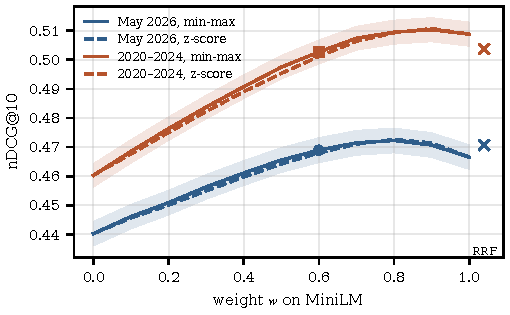
\includegraphics[width=\columnwidth]{hybrid_weights.pdf}
\caption{nDCG@10 of $w\,\hat{s}_{\mathrm{MiniLM}}+(1-w)\,\hat{s}_{\mathrm{BM25}}$ on the test sets ($w=0$: BM25 only, $w=1$: MiniLM only). Solid: min-max, dashed: z-score normalization; bands: 95\% intervals; dots: the pre-specified $w=0.6$; crosses: RRF.}
\label{fig:weights}
\end{figure}

\subsection{Problem-level reading}

Table~\ref{tab:reader} compares reader P@5 with category P@5 on the ten judged queries. \val{reader.sentence}

\begin{table}[!t]
\centering
\caption{Problem-level reading of 10 May-2026 test queries (one annotator, blind to system and category). Reader P@5: same research problem. Category P@5: same primary category, same lists. Right: the 50 top-five slots of each system split by the two labels.}
\label{tab:reader}
\scriptsize
\setlength{\tabcolsep}{2.6pt}
\begin{tabular}{@{}lcccccc@{}}
\toprule
 & Reader & Category & \multicolumn{4}{c}{Slots (problem / category)} \\
\cmidrule(l){4-7}
Method & P@5 & P@5 & yes/yes & yes/no & no/yes & no/no \\
\midrule
BM25 & 0.18 & 0.40 & 3 & 6 & 17 & 24 \\
TF-IDF & 0.20 & 0.36 & 6 & 4 & 12 & 28 \\
LSA & 0.10 & 0.44 & 2 & 3 & 20 & 25 \\
MiniLM & 0.10 & 0.62 & 1 & 4 & 30 & 15 \\
SPECTER2 & 0.10 & 0.52 & 1 & 4 & 25 & 20 \\
BGE-small & 0.16 & 0.54 & 3 & 5 & 24 & 18 \\
Hybrid (0.6) & 0.20 & 0.56 & 3 & 7 & 25 & 15 \\
\bottomrule
\end{tabular}
\end{table}


\section{Discussion}

The two corpora differ in time span, topic mix and the share of cross-listed papers, yet the ordering of systems is the same on both: the dense encoders first, BM25 and LSA next, TF-IDF last. The May corpus is therefore not an outlier caused by a three-week window. At the same time the margins are moderate. The best dense encoder improves category P@5 over the best sparse baseline by \val{gap.points} points on the May corpus and \val{gap.points.y} points on the 2020--2024 corpus, and the per-category split shows that the gain is concentrated in categories whose vocabulary is shared with other fields. A domain-specific encoder helps only slightly: SPECTER2 is ahead of the general-purpose MiniLM by about one point.

The problem-level reading qualifies the main tables. Category agreement counts same-problem papers filed elsewhere as misses and counts different-problem papers in the same category as hits, and on the judged queries the second error is much more frequent. The dense encoders are good at returning papers from the same area, which is what the category proxy rewards, but on these queries a paper about the same specific problem was more often found by term matching: such papers tend to share rare task, dataset or model names with the query. Category precision is useful for comparing systems on thousands of queries, because it is independent of the systems and cheap, but it should not be read as the share of results a researcher would keep, and it may overstate the benefit of dense retrieval for problem-level search. Ten queries are too few to rank systems by reader precision; the reading shows the size of the gap between the two notions of relevance, not a reversed ranking.

\textit{Limitations.} The relevance label is a proxy, and the problem-level check covers 10 queries and one annotator, so it estimates the direction and rough size of the disagreement rather than precise reader precision. Both corpora come from four arXiv computer-science categories and contain titles and abstracts only, so the results do not cover full text, citation graphs or other disciplines. The dense encoders were used off the shelf; fine-tuning or larger models may change the margins. Two weekly windows of January 2024 are missing from the multi-year corpus because of API rate limits.

\section{Conclusion}

On two arXiv computer-science corpora, with every eligible paper used as a query and the query removed from its own results, pretrained dense encoders retrieve more same-category papers than BM25, TF-IDF and LSA. The advantage holds over three weeks of 2026 and over five years of 2020--2024, survives tuning of the sparse baselines on held-out queries, and is statistically reliable, although moderate in size. Mixing BM25 into a dense score with a tuned weight neither helps nor hurts category precision; a fixed weight of 0.6 can hurt it slightly. A blind problem-level reading of ten queries finds low same-problem precision for all systems and no dense advantage, which argues for reporting category precision together with problem-level judgments and for keeping a lexical component in similar-paper search. Future work will add expert judgments from several annotators and full-text and citation signals.

\section*{Data and Code Availability}
\label{sec:availability}
The collection and evaluation scripts, the arXiv identifiers of both corpora, the development and test query lists, per-query scores, rankings and the manual labels are available at \url{https://github.com/Armani7777/arxiv-similar-paper-retrieval}.

\section*{Acknowledgment}
The authors thank arXiv for open access to its metadata. \val{ai.disclosure}

\begin{thebibliography}{99}
\bibitem{batyrkhanov2022intelligent}
A.~G. Batyrkhanov, Zh.~B. Sadirmekova, M.~A. Sambetbayeva, A.~N. Nurgulzhanova, Zh.~S. Ismagulova, and A.~S. Yerimbetova, ``Development of methods and technologies for creating intelligent scientific and educational internet resources,'' \emph{Bull. Electr. Eng. Inform.}, vol.~11, no.~5, pp.~2968--2977, 2022, doi: 10.11591/eei.v11i5.3075.

\bibitem{serikbayeva2021access}
S.~Serikbayeva, J.~Tussupov, M.~Sambetbayeva, A.~Yerimbetova, Zh.~Sadirmekova, A.~Tungatarova, A.~Batyrkhanov, and A.~Zakirova, ``Development of a model and technology of access to documents in scientific and educational activities,'' \emph{East.-Eur. J. Enterp. Technol.}, vol.~6, no.~2(114), pp.~44--58, 2021, doi: 10.15587/1729-4061.2021.248506.

\bibitem{robertson2009bm25}
S.~Robertson and H.~Zaragoza, ``The probabilistic relevance framework: BM25 and beyond,'' \emph{Found. Trends Inf. Retr.}, vol.~3, no.~4, pp.~333--389, 2009.

\bibitem{salton1988term}
G.~Salton and C.~Buckley, ``Term-weighting approaches in automatic text retrieval,'' \emph{Inf. Process. Manage.}, vol.~24, no.~5, pp.~513--523, 1988.

\bibitem{deerwester1990lsa}
S.~Deerwester, S.~T. Dumais, G.~W. Furnas, T.~K. Landauer, and R.~Harshman, ``Indexing by latent semantic analysis,'' \emph{J. Amer. Soc. Inf. Sci.}, vol.~41, no.~6, pp.~391--407, 1990.

\bibitem{reimers2019sbert}
N.~Reimers and I.~Gurevych, ``Sentence-BERT: Sentence embeddings using Siamese BERT-networks,'' in \emph{Proc. EMNLP-IJCNLP}, 2019, pp.~3982--3992.

\bibitem{cohan2020specter}
A.~Cohan, S.~Feldman, I.~Beltagy, D.~Downey, and D.~S. Weld, ``SPECTER: Document-level representation learning using citation-informed transformers,'' in \emph{Proc. ACL}, 2020, pp.~2270--2282.

\bibitem{thakur2021beir}
N.~Thakur, N.~Reimers, A.~R{\"u}ckl{\'e}, A.~Srivastava, and I.~Gurevych, ``BEIR: A heterogeneous benchmark for zero-shot evaluation of information retrieval models,'' in \emph{Proc. NeurIPS Datasets and Benchmarks Track}, 2021.

\bibitem{muennighoff2023mteb}
N.~Muennighoff, N.~Tazi, L.~Magne, and N.~Reimers, ``MTEB: Massive text embedding benchmark,'' in \emph{Proc. EACL}, 2023, pp.~2014--2037.

\bibitem{medic2022large}
Z.~Medi{\'c} and J.~{\v{S}}najder, ``Large-scale evaluation of transformer-based article encoders on the task of citation recommendation,'' in \emph{Proc. 3rd Workshop Scholarly Document Processing}, 2022, pp.~19--31.

\bibitem{mysore2021csfcube}
S.~Mysore, T.~O'Gorman, A.~McCallum, and H.~Zamani, ``CSFCube: A test collection of computer science research articles for faceted query by example,'' in \emph{Proc. NeurIPS Datasets and Benchmarks Track}, 2021.

\bibitem{kreutz2022survey}
C.~K. Kreutz and R.~Schenkel, ``Scientific paper recommendation systems: A literature review of recent publications,'' \emph{Int. J. Digit. Libr.}, vol.~23, no.~4, pp.~335--369, 2022.

\bibitem{pinedo2025survey}
I.~Pinedo, M.~Larra{\~n}aga, and A.~Arruarte, ``Recent advances and trends in research paper recommender systems: A comprehensive survey,'' arXiv:2508.08828, 2025.

\bibitem{ostendorff2022scincl}
M.~Ostendorff, N.~Rethmeier, I.~Augenstein, B.~Gipp, and G.~Rehm, ``Neighborhood contrastive learning for scientific document representations with citation embeddings,'' in \emph{Proc. EMNLP}, 2022, pp.~11670--11688.

\bibitem{singh2023scirepeval}
A.~Singh, M.~D'Arcy, A.~Cohan, D.~Downey, and S.~Feldman, ``SciRepEval: A multi-format benchmark for scientific document representations,'' in \emph{Proc. EMNLP}, 2023, pp.~5548--5566.

\bibitem{mysore2022aspire}
S.~Mysore, A.~Cohan, and T.~Hope, ``Multi-vector models with textual guidance for fine-grained scientific document similarity,'' in \emph{Proc. NAACL}, 2022, pp.~4453--4470.

\bibitem{ajith2024litsearch}
A.~Ajith, M.~Xia, A.~Chevalier, T.~Goyal, D.~Chen, and T.~Gao, ``LitSearch: A retrieval benchmark for scientific literature search,'' in \emph{Proc. EMNLP}, 2024, pp.~15068--15083.

\bibitem{enevoldsen2025mmteb}
K.~Enevoldsen \emph{et~al.}, ``MMTEB: Massive multilingual text embedding benchmark,'' in \emph{Proc. ICLR}, 2025.

\bibitem{xiao2024cpack}
S.~Xiao, Z.~Liu, P.~Zhang, N.~Muennighoff, D.~Lian, and J.-Y. Nie, ``C-Pack: Packed resources for general Chinese embeddings,'' in \emph{Proc. 47th Int. ACM SIGIR Conf. Res. Develop. Inf. Retr.}, 2024.

\bibitem{wang2020minilm}
W.~Wang, F.~Wei, L.~Dong, H.~Bao, N.~Yang, and M.~Zhou, ``MiniLM: Deep self-attention distillation for task-agnostic compression of pre-trained transformers,'' in \emph{Proc. NeurIPS}, 2020, pp.~5776--5788.

\bibitem{luan2021sparse}
Y.~Luan, J.~Eisenstein, K.~Toutanova, and M.~Collins, ``Sparse, dense, and attentional representations for text retrieval,'' \emph{Trans. Assoc. Comput. Linguist.}, vol.~9, pp.~329--345, 2021.

\bibitem{bruch2022fusion}
S.~Bruch, S.~Gai, and A.~Ingber, ``An analysis of fusion functions for hybrid retrieval,'' \emph{ACM Trans. Inf. Syst.}, vol.~42, no.~1, 2024.

\bibitem{cormack2009rrf}
G.~V. Cormack, C.~L.~A. Clarke, and S.~B{\"u}ttcher, ``Reciprocal rank fusion outperforms Condorcet and individual rank learning methods,'' in \emph{Proc. 32nd Int. ACM SIGIR Conf. Res. Develop. Inf. Retr.}, 2009, pp.~758--759.

\bibitem{lin2021pyserini}
J.~Lin, X.~Ma, S.-C. Lin, J.-H. Yang, R.~Pradeep, and R.~Nogueira, ``Pyserini: A Python toolkit for reproducible information retrieval research with sparse and dense representations,'' in \emph{Proc. 44th Int. ACM SIGIR Conf. Res. Develop. Inf. Retr.}, 2021, pp.~2356--2362.

\bibitem{smucker2007significance}
M.~D. Smucker, J.~Allan, and B.~Carterette, ``A comparison of statistical significance tests for information retrieval evaluation,'' in \emph{Proc. 16th ACM Conf. Inf. Knowl. Manage. (CIKM)}, 2007, pp.~623--632.

\bibitem{holm1979}
S.~Holm, ``A simple sequentially rejective multiple test procedure,'' \emph{Scand. J. Statist.}, vol.~6, no.~2, pp.~65--70, 1979.

\end{thebibliography}

\end{document}
